\chapter{Introduction}\label{chapter:introduction}

Number theory is the study of numbers, particularly the natural numbers (the numbers $0,1,2,\ldots$ increasing indefinitely in increments of $1$), the integers (the numbers $\ldots, -2, -1, 0, 1, 2, \ldots$), and occasionally the rational numbers (fractions of integers). Its central themes include questions about divisibility, prime numbers, modular arithmetic, arithmetic functions, and finding integer solutions to equations. Additionally, number theory explores combinatorial questions, such as determining how numbers can be decomposed into sums or products of specific forms, like squares or primes. More advanced branches of number theory are occasionally also concerned with the properties of other number systems, such as the real numbers, complex numbers, or $p$-adic numbers. However, in \emph{elementary number theory} these explorations are primarily motivated by how these number systems relate back to the integers.

\section*{A Short History of Number Theory}

\begin{wrapfigure}[19]{r}{0.35\textwidth}
  \centering
  \begin{tikzpicture}
    \node[inner sep=0pt, rounded corners=0.2em, clip] {%
      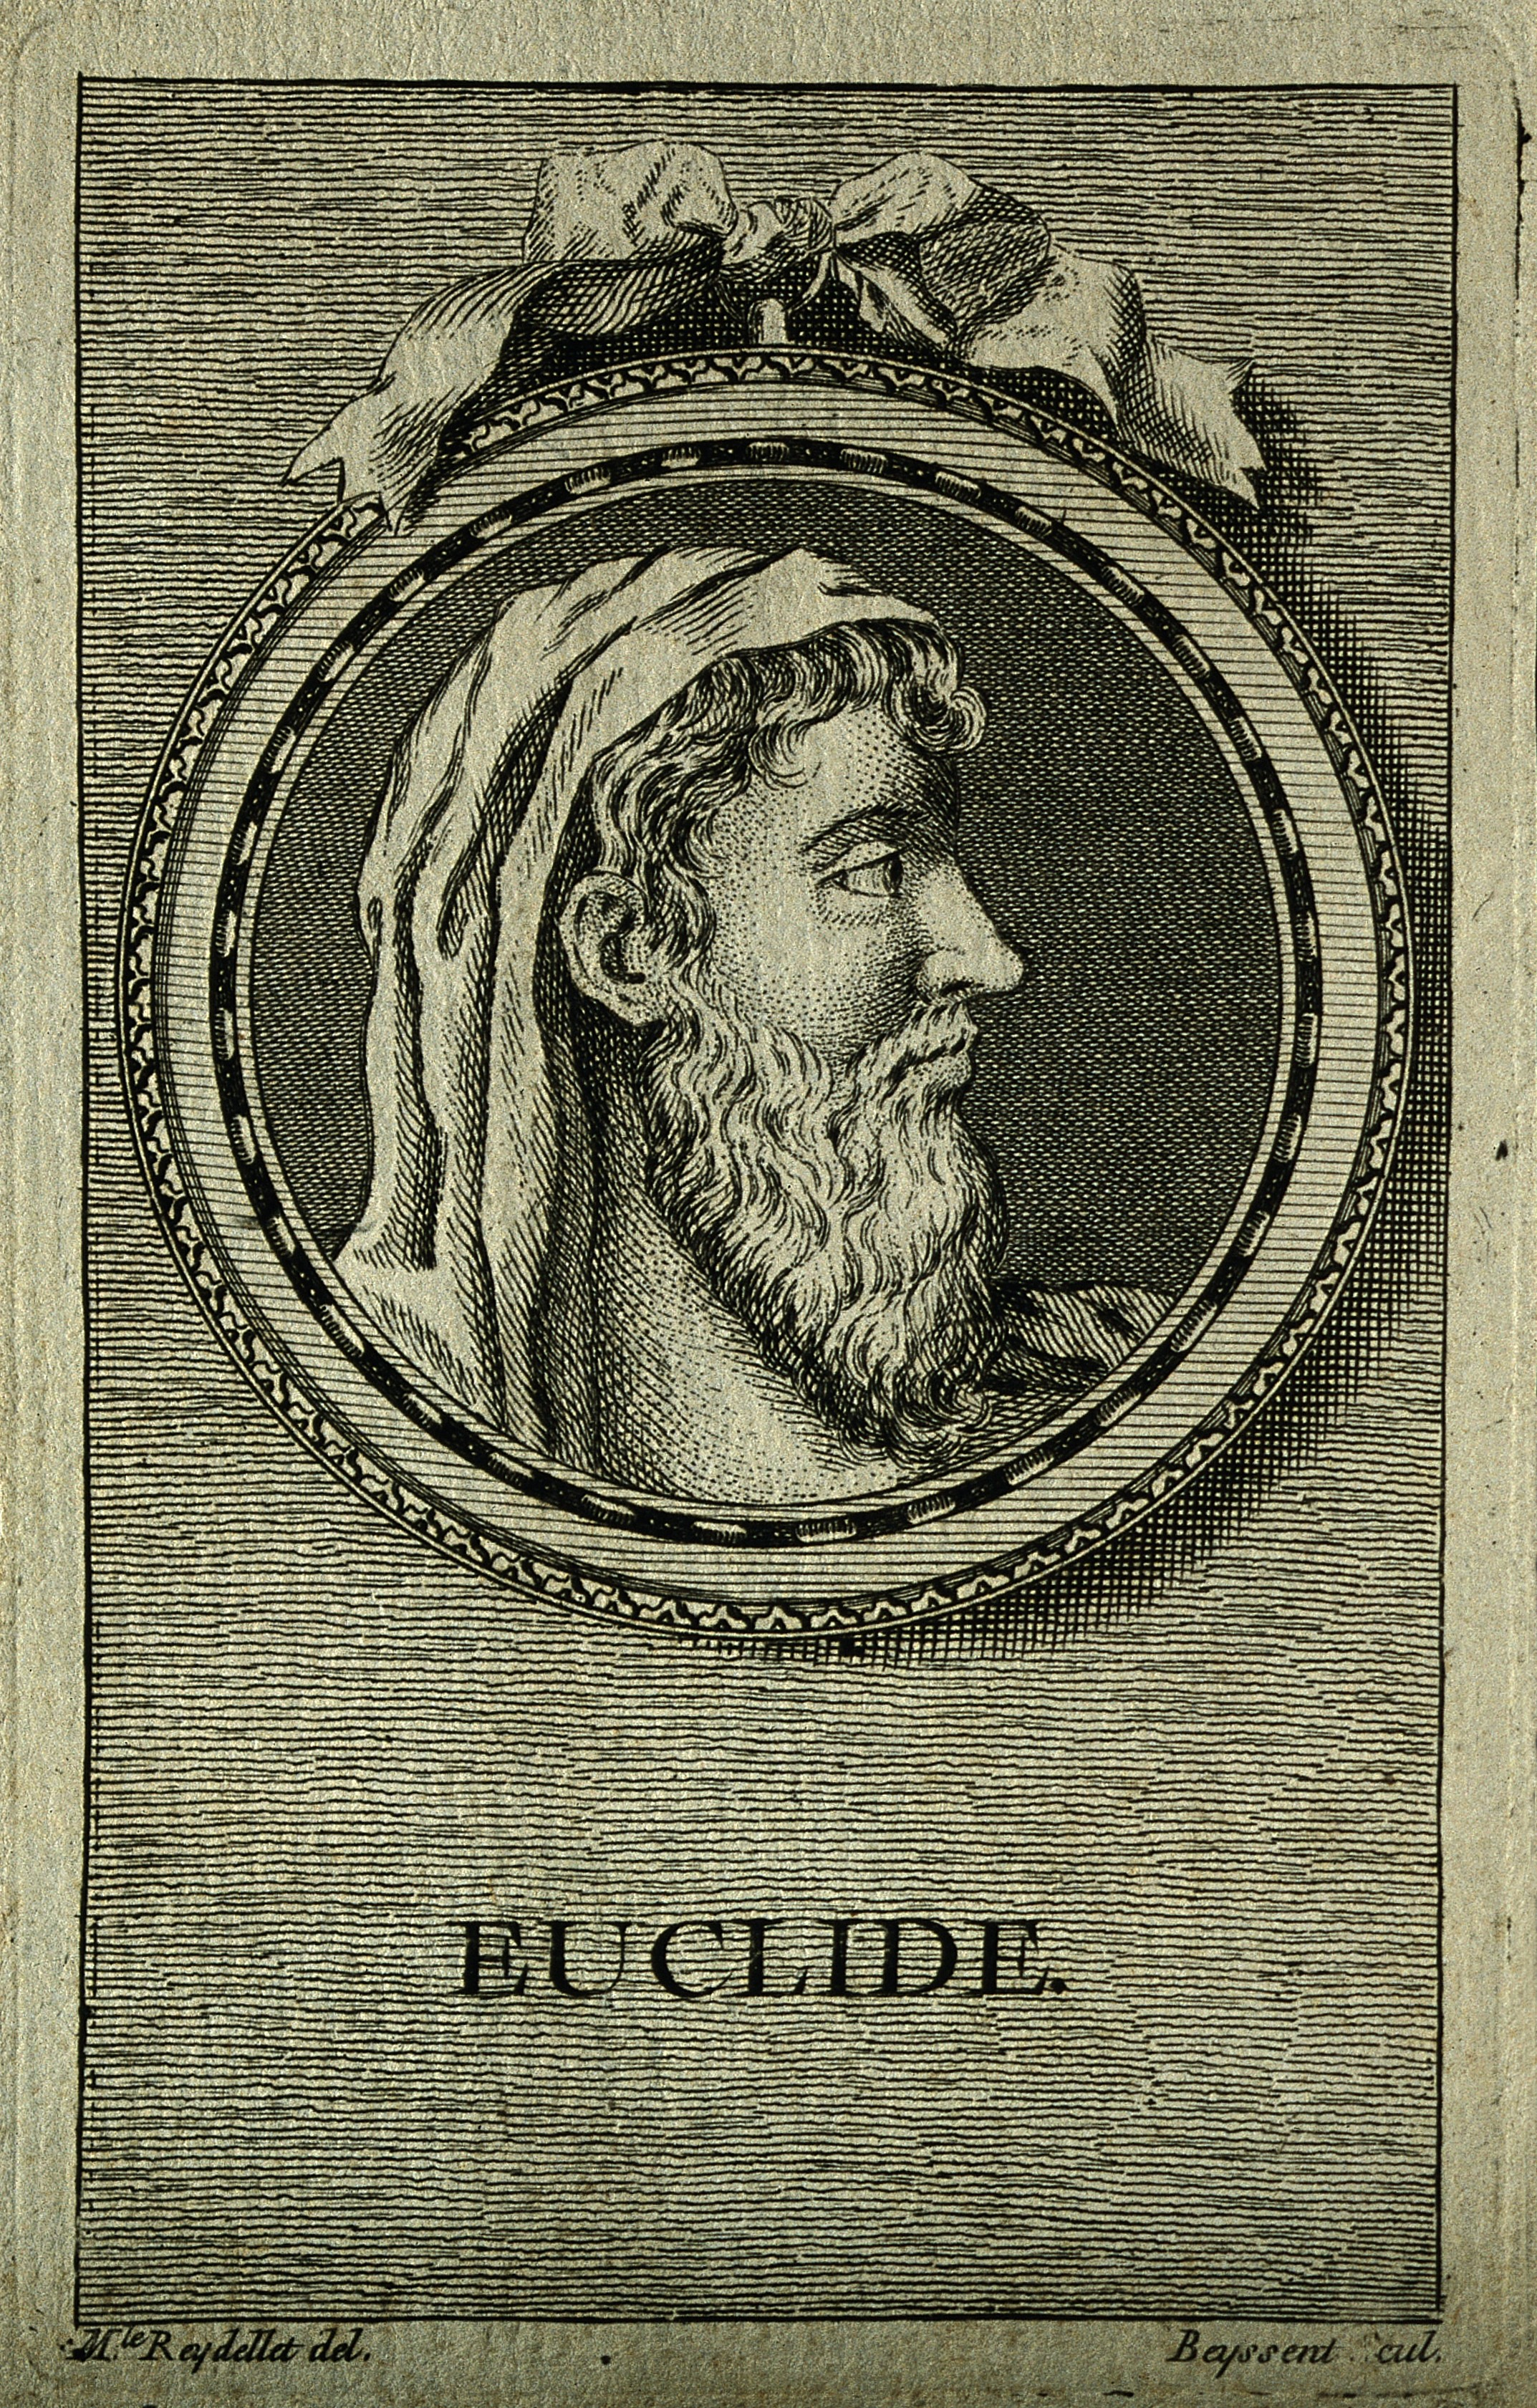
\includegraphics[width=0.3\textwidth]{Euclid-Beyssent-line-engraving.jpg}%
    };
  \end{tikzpicture}
  \caption{Line engraving by S. Beyssent after Mlle. C. Reydell}
  \label{fig:euclid}
\end{wrapfigure}
Number theory has a long history that dates back to antiquity. One of the earliest and most influential systematic treatments of mathematics is Euclid's Elements \cite{euclid1908}, written around 300 BC in Alexandria. In this work, Euclid established several key results in number theory, including the infinitude of primes and the algorithm for finding the greatest common divisor, which bears his name.

Around 250 AD, the Greek mathematician Diophantus of Alexandria wrote his \emph{Arithmetica} \cite{diophantus1910}, which focused on solving what are now known as Diophantine equations. This 13-volume work is often considered the first comprehensive treatment of algebra, though Diophantus relied on rhetorical descriptions rather than modern algebraic notation. Only six of the original volumes have survived, but they profoundly influenced later mathematicians.

The works of Euclid and Diophantus were preserved and studied by scholars in the Byzantine Empire, such as Theon of Alexandria and his daughter Hypatia. They added commentaries that clarified and expanded upon the original text.

During the Islamic Golden Age, scholars like Al-Khwarizmi, Ibn al-Haytham, and Omar Khayyam preserved and expanded upon the works of Euclid and Diophantus. Al-Khwarizmi’s work, especially his \emph{Kitab al-Mukhtasar fi Hisab al-Jabr wal-Muqabala} (from which the term "algebra" originates), introduced systematic methods for solving linear and quadratic equations. He used rhetorical algebra, like Diophantus, but began a transition toward symbolic representation by relying on consistent terminology for operations and equations.

After the invention of the printing press, Erhard Ratdolt, a German printer based in Venice, produced the first printed edition of the Elements in 1482. This edition included mathematical diagrams and marked an important step in the dissemination of Euclid’s work. The first printed edition of Diophantus' Arithmetica was published in 1575 by Wilhelm Xylander, a German mathematician. The printing was done in Basel, Switzerland, a major hub for academic publishing at the time. By the time of Pierre de Fermat in the 17th century, both the Elements and Arithmetica had become essential texts for mathematicians across Europe, influencing the development of number theory and inspiring Fermat’s groundbreaking contributions.

\begin{wrapfigure}[21]{r}{0.4\textwidth}
  \centering
  \begin{tikzpicture}
    \node[inner sep=0pt, rounded corners=0.2em, clip] {%
      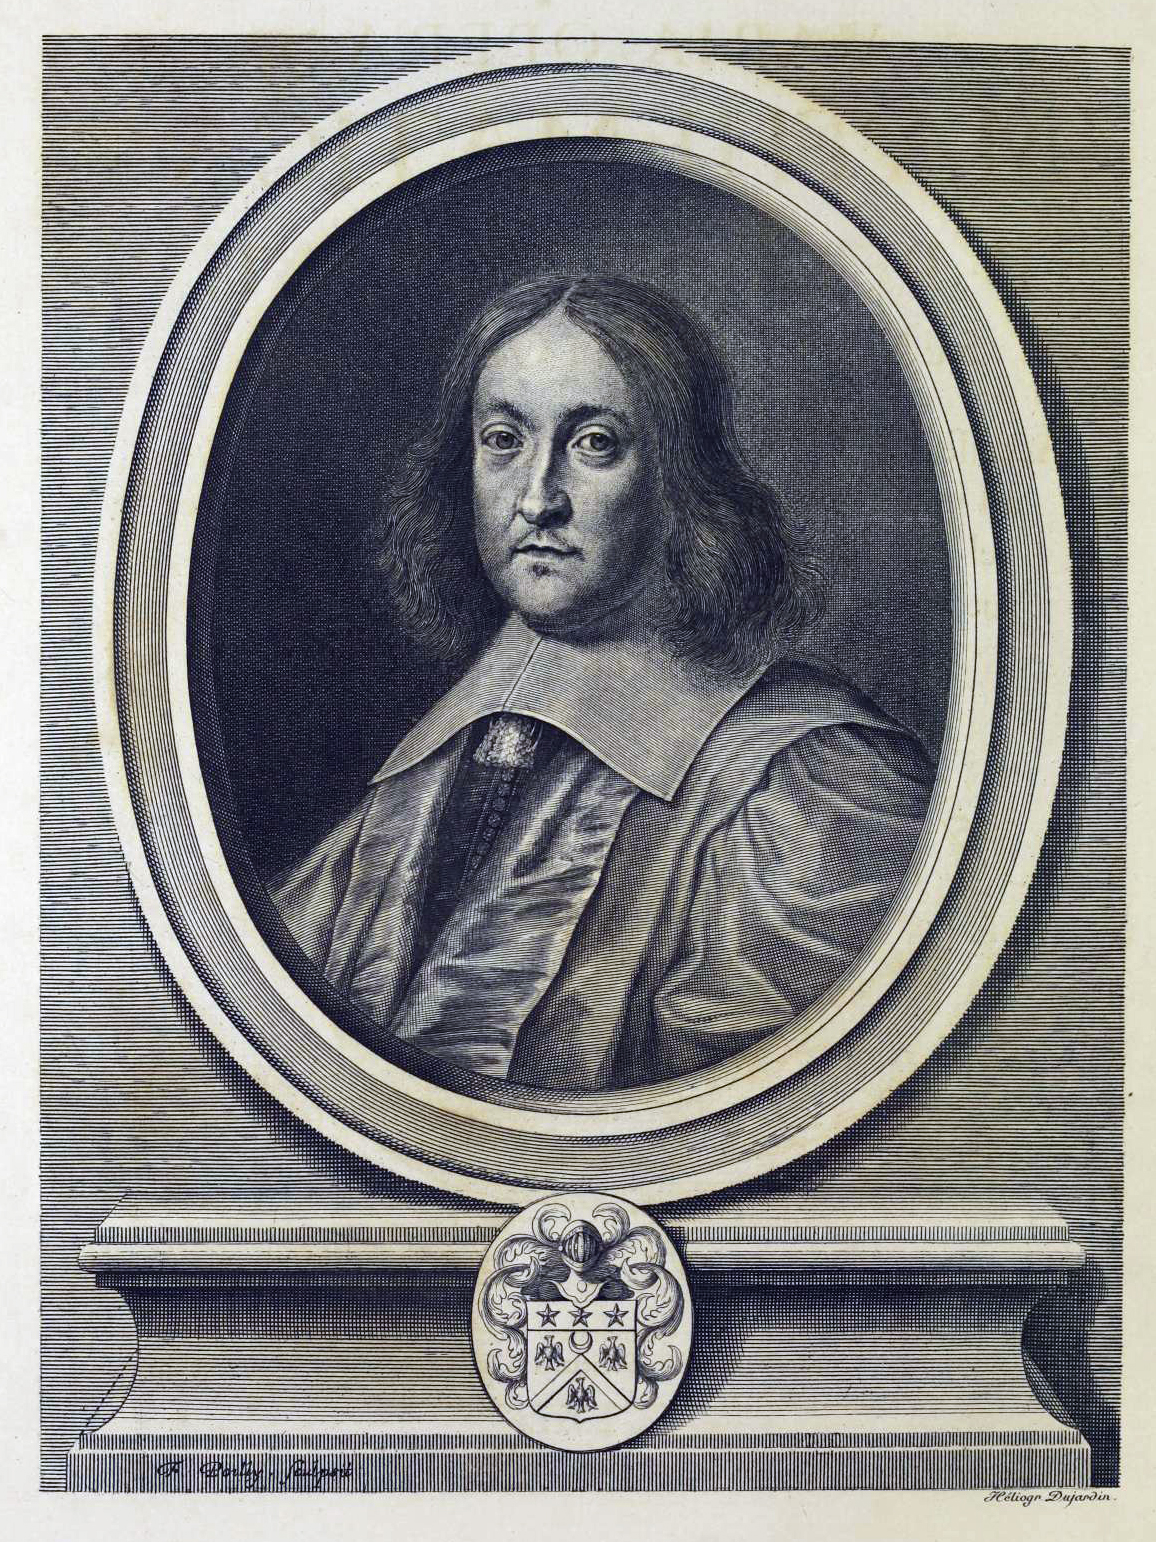
\includegraphics[width=0.38\textwidth]{Fermat.jpg}%
    };
    \end{tikzpicture}
    \caption{Pierre de Fermat. Engraving in Oeuvres Mathématiques Diverses.}
  \label{fig:fermat}
\end{wrapfigure}

Pierre de Fermat (1607–1665) is often considered the founder of modern number theory. He was a contemporary of Blaise Pascal and Marin Mersenne, both of whom he corresponded with, and also of Galileo Galilei. He wrote a manuscript titled \emph{Éléments de Géométrie}, which served as an extension and commentary on Euclid’s Elements. In this work, he sought to modernize Euclid’s geometry by applying the emerging methods of algebra and analytic geometry to classical geometric problems.

Fermat made several groundbreaking contributions to number theory. He proved \emph{Fermat's Little Theorem}, which is a central theorem of this course, and he formulated the \emph{sum of two squares theorem} asserting that an odd prime $p$ can be expressed as the sum of two squares if and only if $p\equiv 1\pmod{4}$. He also introduced the method of \emph{infinite descent}, and formulated the \emph{Polygonal Number Theorem}, which states that every positive integer can be expressed as the sum of at most $n$ $n$-gonal numbers.

Fermat also made several famous conjectures. He conjectured that the equation $x^2+Ny^2=1$ has infinitely many solutions for any non-square integer $N$. Euler made a significant advance to this problem by proving it for specific values of $N$. The general form of the solution to equations of the form $x^2+Ny^2=1$ was found later by Legendre and Lagrange.

Finally, Fermat famously asserted that there could be no three nonzero integers $x$, $y$, and $z$ such that the equation
\begin{equation*}
  x^n+y^n=z^n
\end{equation*}
holds, when $n\geq 3$. This statement is now known as \emph{Fermat's Last Theorem}. He claimed to have a "truly marvelous proof", but that the margin of his copy of \emph{Arithmetica} was too small to contain it. His assertion, known as \emph{Fermat’s Last Theorem}, captivated mathematicians for centuries. It was finally proven in 1995 by Andrew Wiles, about 350 years after Fermat made his famous note in the margin, using advanced techniques from algebraic geometry and modular forms. Wiles’s achievement is considered one of the most remarkable milestones in the history of mathematics.

While Fermat laid the groundwork for modern number theory, we should mention that the concept of \emph{function} hasn't been crystallized until Leibniz coined the term in 1673, using it to describe quantities related to curves, such as slopes, tangents, and areas. Bernoulli played a significant role in expanding the idea of functions. He used the term explicitly in 1718, describing it as a quantity dependent on another variable. Euler provided the first modern definition of a function in his \emph{Introductio in Analysin Infinitorum} (1748) \cite{euler1988}. He emphasized that functions could include both algebraic (e.g., polynomials) and transcendental forms (e.g., trigonometric and exponential functions). Peter Gustav Lejeune Dirichlet was the first to define functions abstractly as a correspondence between two sets, removing the requirement for expressions or formulas. This abstraction was a key insight for the theorem that we now know as \emph{Dirichlet's theorem}: Every arithmetic progression
\begin{equation*}
  a,\ a+b,\ a+2b,\ a+3b,\ \ldots
\end{equation*}
\begin{wrapfigure}[21]{r}{0.4\textwidth}
  \centering
  \begin{tikzpicture}
    \node[inner sep=0pt, rounded corners=0.2em, clip] {%
      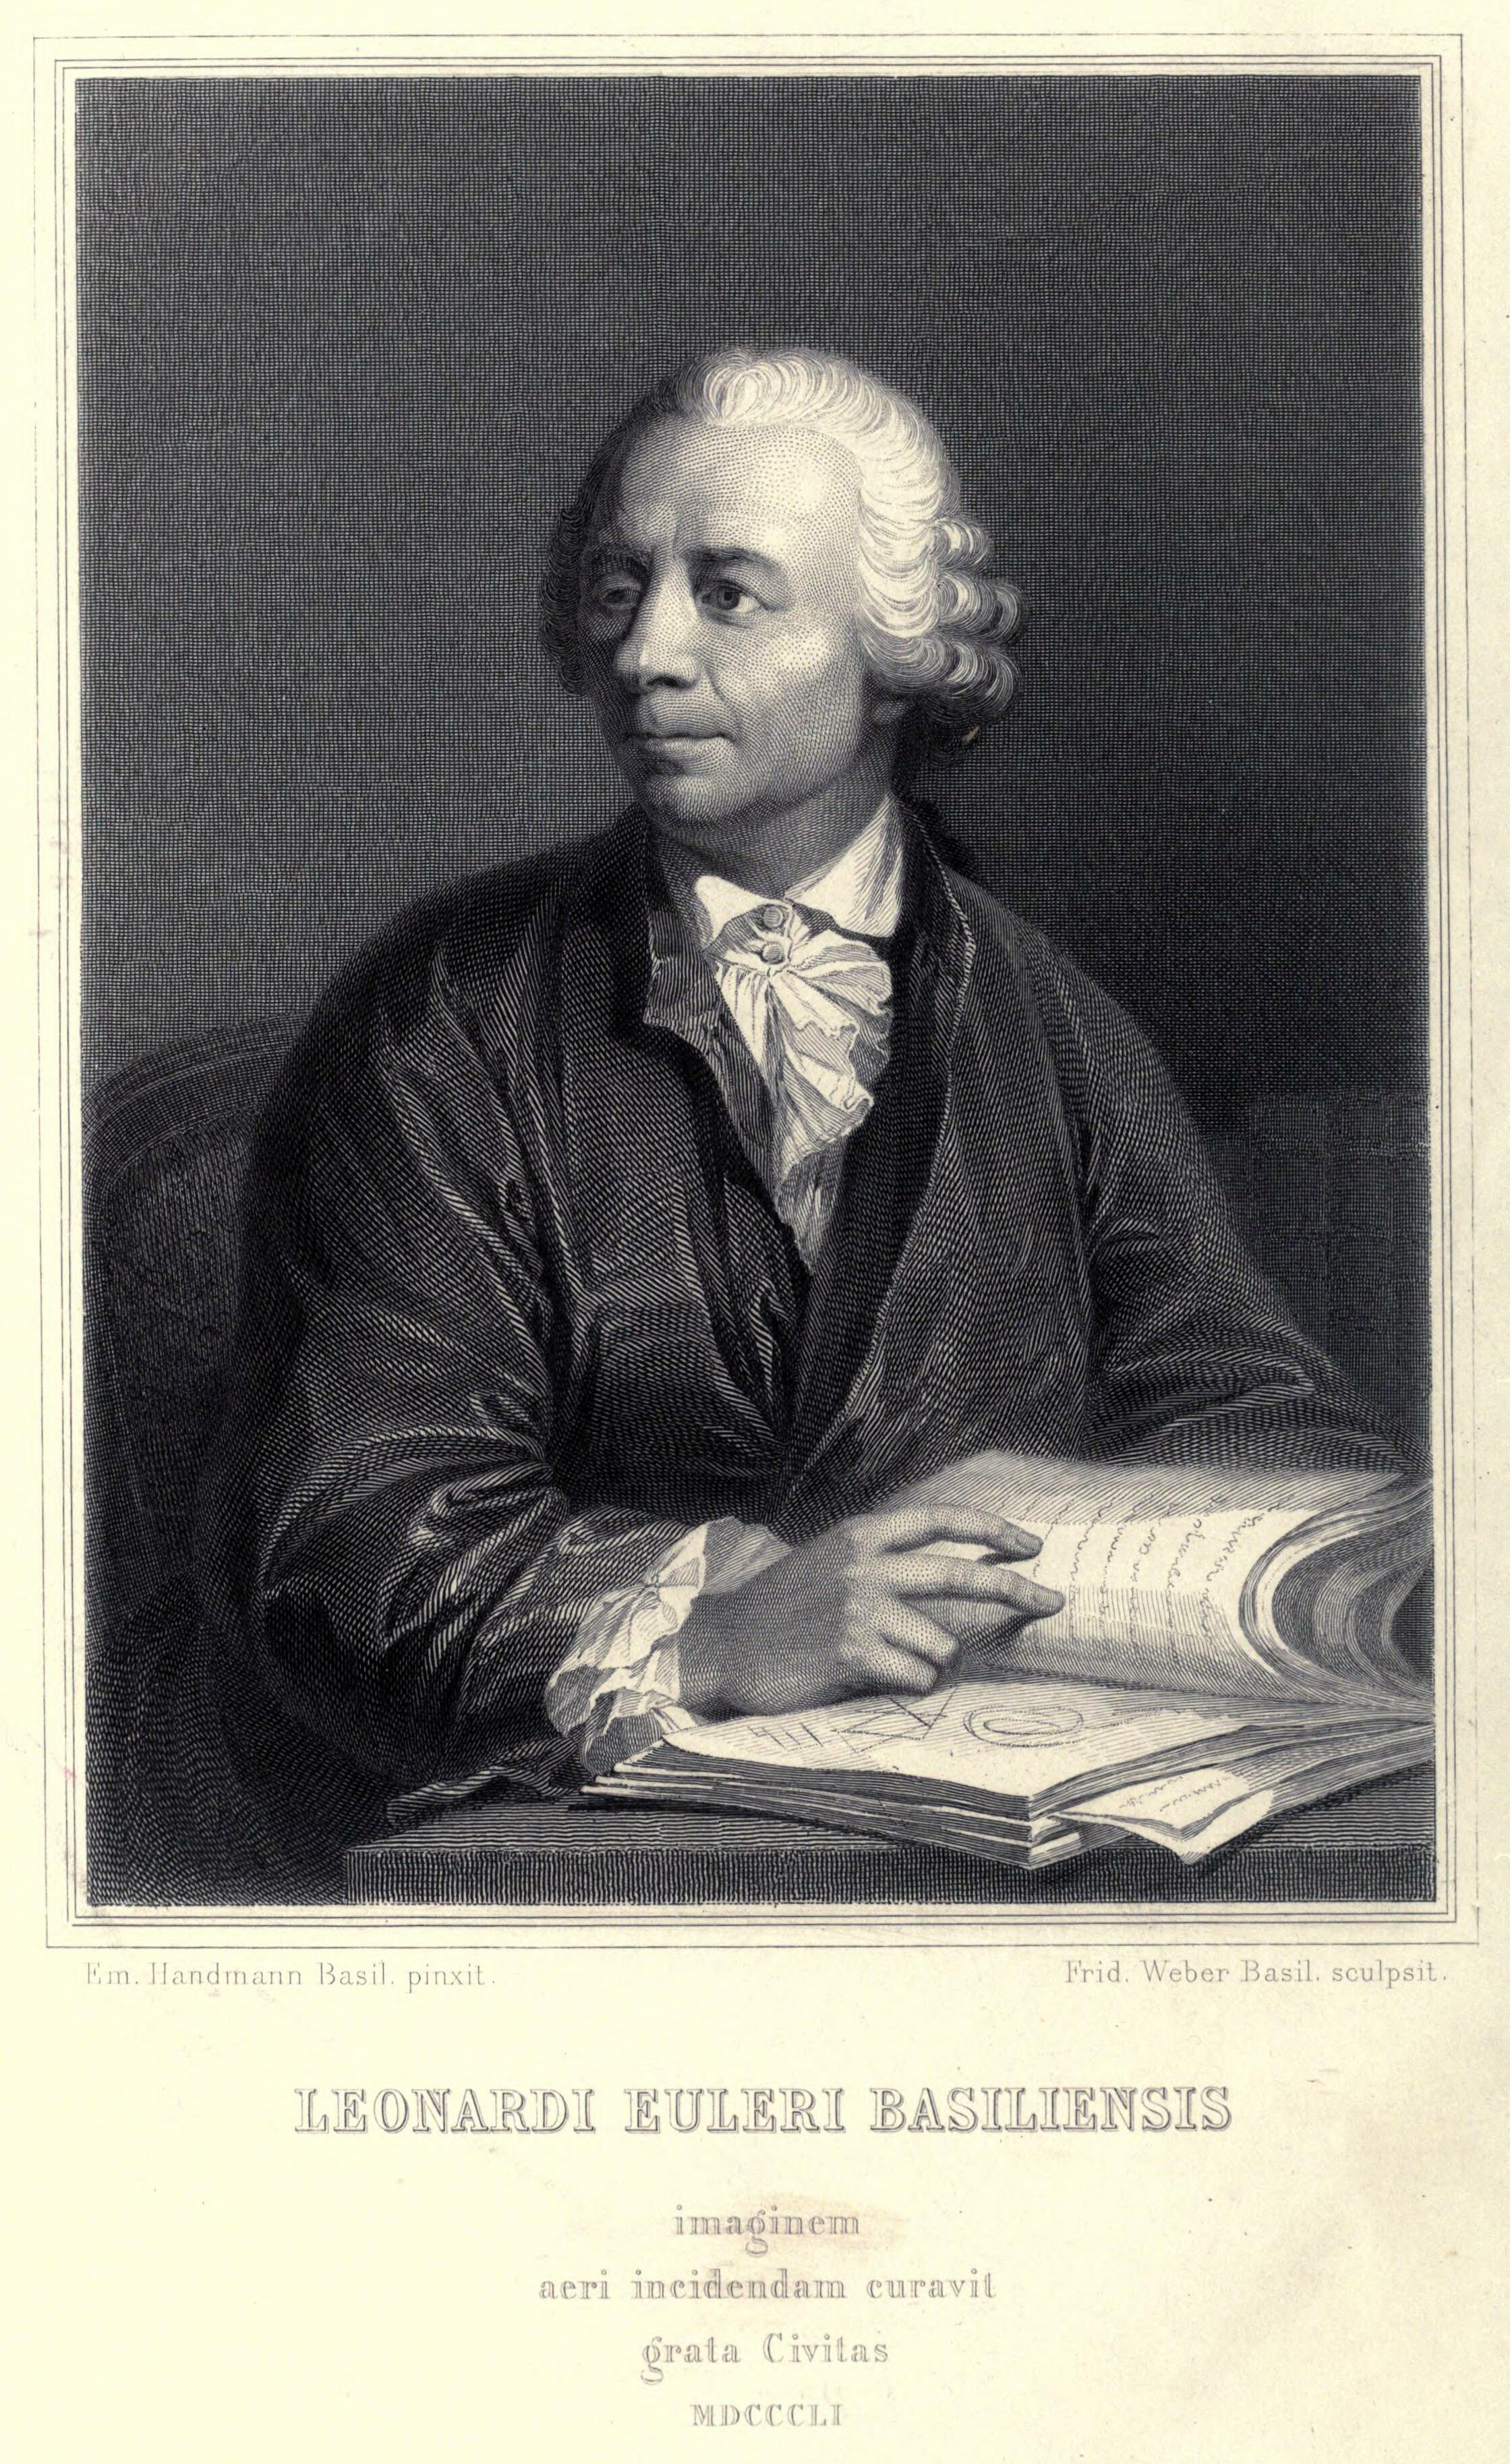
\includegraphics[width=0.38\textwidth]{Euler.jpg}%
    };
  \end{tikzpicture}
  \caption{Leonhard Euler. Engraving by Friedrich Weber.}
  \label{fig:euler}
\end{wrapfigure}
in which $a$ and $b$ are coprime, contains an infinitude of primes. Dirichlet proved his theorem in 1837, more than 150 years after Leibniz first coined the term of function.

Euler's Introductio in Analysin Infinitorum marked the beginning of \emph{analytical number theory}. As we mentioned before, Euler defined functions here and established the notation $f(x)$ of a function applied to its variable, which we still use today. He derived the famous formula for complex exponentials
\begin{equation*}
  e^{ix}=\cos(x) + i \sin(x).
\end{equation*}
This identity connects the exponential function, trigonometric functions, and the imaginary unit. The Riemann zeta function $\zeta(s)$ makes its first appearance here in a complex variable $s$, and he derived the celebrated \emph{product formula}
\begin{equation*}
  \zeta(s)=\sum_{n=1}^{\infty}\frac{1}{n^s}=\prod_{p\,\mathrm{prime}}\frac{1}{1-p^{-s}}.
\end{equation*}
More generally, Euler explored infinite series and products. The \emph{Basel summation formula}
\begin{equation*}
  \sum_{n=1}^\infty \frac{1}{n^2}=\frac{\pi^2}{6}
\end{equation*}
was first proven here, which was one of Euler's most celebrated achievements. Euler was keen to explore the connection between geometry and analysis, and in Introductio in Analysin Infinitorum, he advanced the idea that the study of functions and infinite series could provide new insights into geometric problems. He showed how techniques from analysis could be used to solve problems in geometry and vice versa, fostering the development of applied mathematics.

\begin{wrapfigure}[21]{r}{0.4\textwidth}
  \centering
  \begin{tikzpicture}
    \node[inner sep=0pt, rounded corners=0.2em, clip] {%
      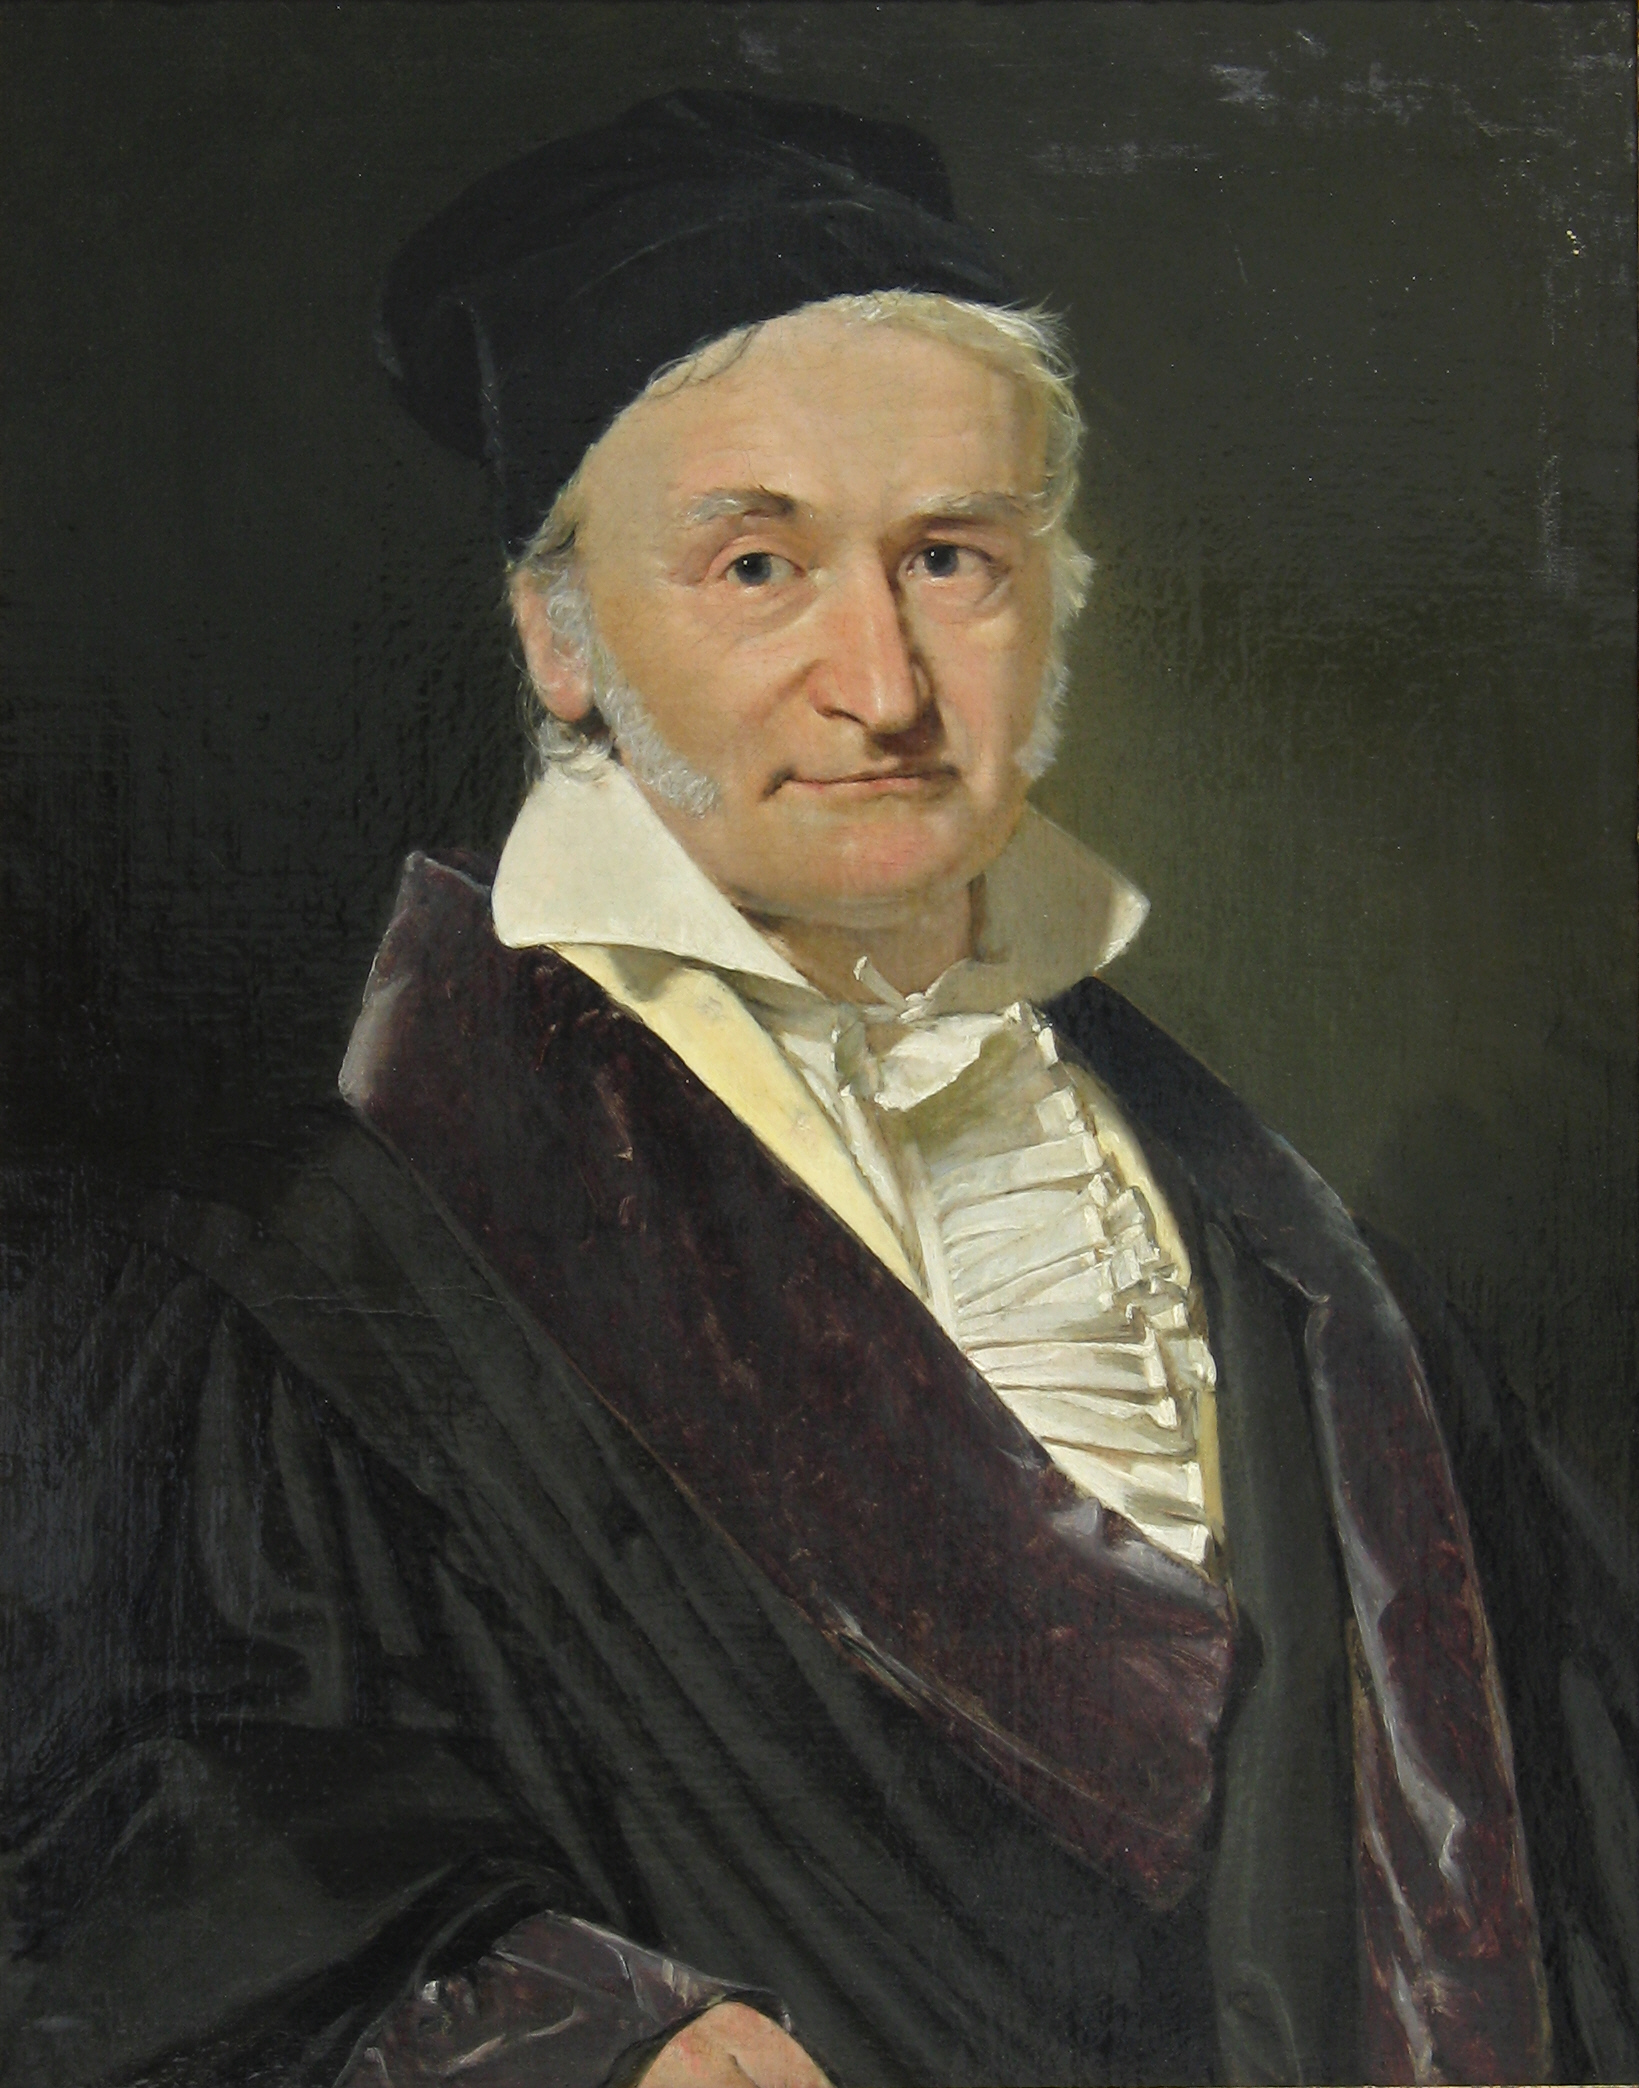
\includegraphics[width=0.38\textwidth]{Gauss.jpg}%
    };
  \end{tikzpicture}
  \caption{\sloppy{Carl Friedrich Gauss. Painting by Christian Albrecht Jensen.}}
  \label{fig:gauss}
\end{wrapfigure}
Building on the work of Euler, Gauss began using the properties of the zeta function and other analytic methods to investigate the distribution of the primes. His seminal work \emph{Disquisitiones Arithmeticae} \cite{gauss1986} is often considered the starting point of the study of the distribution of primes, ultimately leading up to the \emph{Prime Number Theorem}. Gauss conjectured that the number $\pi(n)$ of primes below a number $n$ satisfies the asymptotic law
\begin{equation*}
  \pi(n)\sim\frac{n}{\log(n)}.
\end{equation*}
This conjecture was proved independently by Jacques Hadamard and Charles Jean de la Vallée Poussin. Furthermore, Gauss laid the foundation for modular arithmetic, and proved the celebrated law of quadratic reciprocity, which tells us when a quadratic equation modulo a prime number is solvable. More precisely, it states that if $q\equiv 1\pmod{4}$ then the congruence $x^2\equiv p \pmod{q}$ is solvable if and only if the congruence $x^2\equiv q\pmod{p}$ is solvable.

So far, we have covered some of the most celebrated advances in humanity's understanding of numbers up to the early 19th century. Mathematics has made rapid progress since then. Bertrand's postulate, which asserts that there is always at least one prime $p$ between $n$ and $2n$, for any $n>1$, was proven by Pafnuty Chebyshev in 1852, and Ben Green and Terence Tau proved in 2004 that the sequence of prime numbers contains arbitrarily long arithmetic progressions.

The 20th century saw the emergence of the Langlands program, a far-reaching research program that aims to connect number theory, representation theory, and algebraic geometry. With the contributions of mathematicians like André Weil, Robert Langlands, and many others, the program has shaped much of the direction of modern research in number theory and its applications to other branches of mathematics.

Even today fundamental concepts such as sets and functions continue to evolve. We live in an era of digital computation, with tools far beyond the reach of Fermat, Euler, and Gauss, where essentially all recorded knowledge is readily available to almost anyone. This computational revolution has also given rise to powerful tools like proof assistants—computer programs designed to construct and formally verify mathematical proofs. Since proof assistants are programming languages, they are often based on type theory rather than set theory, slightly changing the way mathematics is done. Functions in type theory are even more general than Leibniz, Euler, and Dirichlet envisioned: unlike in set theory where functions are a specific kind of relations between sets, functions in type theory are primitive entities satisfying certain rules for evaluation, and they have an extra dependency built in, allowing types of their outputs to depend on the input. Proof assistants are being used with great success to formally verify advanced mathematical theorems. Georges Gonthier formally verified the Four Color Theorem and the Odd Order Theorem, and Tom Hales verified Kepler's conjecture about sphere packings. A current effort led by Kevin Buzzard aims to formally verify Fermat's Last Theorem.

Today, number theory continues to be one of the most active and fruitful areas of mathematical research, all of which started simply with counting on ten fingers.

\section*{Overview of the Course}

An integer $a$ is said to \emph{divide} an integer $b$ if there exists an integer $x$ such that $ax=b$. In other words, the number $a$ divides $b$ if the equation
\begin{equation*}
  ax=b  
\end{equation*}
has a solution in the integers. In this case we say that $a$ is a \emph{divisor} of $b$, and we write $a \mid b$. This equation is the simplest example of a Diophantine equation. Diophantine equations are equations expressed using variables, integers, and arithmetic operations. The primary goal of solving a Diophantine equation is to find integers for each of the variables for which the equation is true. The study of Diophantine equations is a cornerstone of number theory.

For example, the equation
\begin{equation*}
  x^2 - 1 = 0
\end{equation*}
is a \emph{quadratic Diophantine equation} with two solutions: $x=\pm 1$. One of the most well-known quadratic Diophantine equations is the equation
\begin{equation*}
  x^2 + y^2 = z^2,
\end{equation*}
which is a Diophantine equation in \emph{three variables}. Its solutions are known as \emph{Pythagorean triples}. These triples, such as $(3,4,5)$ and $(5,12,13)$, corresponds to the side lengths of right-angled triangles and have been studied since antiquity. Perhaps the most famous Diophantine equation is Fermat's equation
\begin{equation*}
  x^n + y^n = z^n,
\end{equation*}
which has no solutions for nonzero integers $x$, $y$, and $z$ when $n\geq 3$.

In this course, however, we will not go as far as proving Fermat's last theorem. The first target of this course is the Fundamental Theorem of Arithmetic, which establishes the prime numbers as the building blocks of all natural numbers. A number $n$ is said to be prime if it has exactly one divisor $d \mid n$ such that $d\neq n$. If this is the case, then its unique divisor that is not equal to itself is the number $1$. The Fundamental Theorem of Arithmetic asserts that any nonzero natural number $n$ can be written as a product of primes
\begin{equation*}
  n=p_1p_2\cdots p_k,
\end{equation*}
and that this decomposition of $n$ as a product of primes is unique up to the ordering of the primes.

In order to study divisibility properties more deeply, Gauss introduced in his \emph{Disquisitiones Arithmeticae} the congruence relations of modular arithmetic. Following Gauss, we say that a number $a$ is congruent to $b$ modulo $n$, that is,
\begin{equation*}
  a \equiv b \pmod{n}
\end{equation*}
if $n \mid b - a$. Gauss used this new formalism to study quadratic residues, the Chinese Remainder theorem, and a variety of other problems in number theory, a thread we will also pick up on in this course.

Some of the most important theorems in this context are Fermat's Little Theorem, Euler's Theorem, and Wilson's Theorem. Fermat's theorem asserts that given any prime number $p$ and any number $a$ that is not divisible by $p$ we have
\begin{equation*}
  a^{p-1}\equiv 1 \pmod{p}.
\end{equation*}
Fermat's theorem is an important ingredient in primality tests: If the congruence $a^{n-1}\equiv 1 \pmod{n}$ is false then the number $n$ cannot be prime. Testing this congruence for several values of $a$ is a simple way of discovering that $n$ is composite. This test is by itself, however, not conclusive because there are some numbers, the Carmichael numbers, that satisfy Fermat's congruence for all $a$ relatively prime to $n$.

Euler's theorem is a sharper version of Fermat's Little Theorem, but it involves a new function: \emph{Euler's totient function}. Euler's totient function $\phi$ counts the numbers less than $n$ that are relatively prime to $n$, which means that they share no common divisors with $n$ other than $1$. For example, if $p$ is a prime number then $\phi(p)=p-1$ since every number $0<n<p$ is relatively prime to $p$. Using the totient function, Euler's theorem asserts that the congruence relation
\begin{equation*}
  a^{\phi(n)}\equiv 1 \pmod{n}
\end{equation*}
holds for any natural number $n$ and any number $a$ relatively prime to $n$. Euler's theorem has applications in cryptography.

Wilson's Theorem states that a number $p$ is a prime number if and only if the congruence
\begin{equation*}
  (p-1)!\equiv -1 \pmod{p}
\end{equation*}
holds. Here, the exclamation mark is used for the \emph{factorial function}: The number $n!$ is the product $1\cdots n$ of all the numbers from $1$ through $n$. Wilson's Theorem therefore gives another criterion for primality testing.

Euler's totient function is an example of an arithmetic function. Other such functions include the function $\tau(n)$, which returns the number of divisors of a number $n$, the function $\sigma(n)$, which returns the sum of the divisors of a number $n$, and the \emph{M\"obius function} $\mu$. These and other functions have important relations between them, that we will investigate next. The M\"obius inversion formula, for instance, states that if $f$ and $g$ are two arithmetic functions, then we have
\begin{equation*}
  f(n)=\sum_{d\mid n} g(d)\qquad\text{if and only if}\qquad g(n)=\sum_{d\mid n}\mu(d)f\left(\frac{n}{d}\right).
\end{equation*}
This result allows us to "invert" summation relations involving divisors.

The M\"obius inversion is only one aspect of an algebraic structure that is present on the set of all arithmetic functions. Arithmetic functions can be multiplied by an operation known as \emph{Dirichlet convolution}, which gives the set of arithmetic functions the structure of a \emph{commutative ring}. Commutative rings are sets with operations of addition and multiplication satisfying the usual laws of arithmetic, and having such a structure on a set gives us a great opportunity to study them further. In our case, we get to study the primes more closely.

Experimentation is essential in number theory. By making lists of primes, lists of numbers that can be written as the sum of two squares or sums of three squares, lists of square-free numbers, and so on, you will start to gather data on numbers and perhaps start seeing patterns that might otherwise feel elusive. At the end of this section, we have produced two number grids with the numbers from $1$ to $1728$. The great masters all have endlessly created such lists to organize and discover patterns in various kinds of numbers. Feel free to print it as many times as you like, and color them according to your own rules, or whenever something in the course piques your interest. Some exercises throughout the course will ask you to color this number grid in a certain way.

\section*{Literature}
In this course we will be following \cite{andrews1994} fairly closely. One distinctive feature of this book is that it presents many of the most important theorems from two perspectives: a combinatorial one and an abstract one. This dual approach helps to clarify not only why these results are true but also appreciate why they are natural and inevitable within the broader framework of mathematics.

However, there are many excellent sources to learn number theory from. One of my personal favorites for its clarity and accessibility is LeVeque's \emph{Topics in Number Theory} \cite{leveque1956vol1,leveque1956vol2}. Both Andrews' and LeVeque's textbooks contain plenty of exercises, most of which are very fun.

Silverman's \emph{Friendly Introduction to Number Theory} \cite{silverman2012} is another wonderful textbook, explaining the ideas behind many theorems and methods in number theory in a very accessible way, with practical examples and exercises. If you find some parts of Andrews or these notes hard to follow, you may well find the Friendly Introduction very helpful.

The undisputed classic textbook on number theory is Hardy and Wright's \emph{Introduction to the Theory of Numbers} \cite{hardy2008}. This book covers all the essential topics in number theory, including elementary number theory and analytical number theory. It is more comprehensive and also provides more historical notes. The textbook of Hardy and Wright does not provide exercises, but it contains the proofs of many important facts in number theory that are stated as exercises elsewhere.

\section{Online resources}

There are plenty of ways to learn number theory and engage with communities of mathematicians and students online. First and foremost, wikipedia has many excellent pages on topics from and related to number theory. The website math.stackexchange.com is dedicated to answering any kind of mathematical questions, although the more research related questions are usually posed on mathoverflow.net. The website artofproblemsolving.com is dedicated to contest mathematics and the problem solving techniques necessary to do well in competitions such as the International Mathematics Olympiad. Furthermore, there are some popular channels on video sharing sites such as YouTube and TikTok. We mention some of the most popular channels:

Lectures:
\begin{enumerate}
\item Richard Borcherds is a Fields Medalist, and has recorded many of his Berkeley lectures for YouTube. This is a must-watch.
\end{enumerate}

Problem solving:
\begin{enumerate}
\item \textbf{Michael Penn} has an excellent YouTube channel in which he solves interesting mathematical problems on a blackboard, at roughly the level of this course.
\item vEnhance (Evan Chen) is an IMO gold medalist and author of the book \emph{Euclidean Geometry in Math Olympiads} \cite{chen2016}. He streams live solves of olympiand math problems on Twitch and his videos are also available on youtube.\item OmegaLearn is Jonathan Huang's YouTube channel about solving IMO problems. Some of his playlists dive deeper into specific techniques such as Fermat's infinite descent.
\item MindYourDecisions (Presh Talwalkar) presents puzzles and number-theoretic tricks, often with surprising or elegant solutions.
\item Math with Ms. Lin
\item Sokoban’s Den
\item Brent Ferguson’s Math
\end{enumerate}

Mathematics for a broad audience:
\begin{enumerate}
\item \textbf{3Blue1Brown} dives deeply into a variety of topics related to computer science and mathematics with compelling visualizations
\item Mathologer is Burkard Polster's YouTube channel for recreative mathematicians. Many of his videos contain nice visual proofs, especially his videos about Fermat's Two-Square theorem and the quadratic reciprocity theorem are worth watching.
\item Numberphile is a long running YouTube channel of Brady Haran in which mathematicians are interviewed to explain a variety of mathematical phenomena, includin topics related to number theory.
\item Standupmaths
\item Blackpenredpen
\item Tom Rocks Maths
\item @professorpuzzle (TikTok)
\item @numeracynerd (TikTok)
\end{enumerate}

You might also enjoy joining some Discord servers, such as the AoPS community server (Art of problem solving), the Math Stack Exchange Discord, or the OmegaLearn Server.

Finally, you might also find generative AI useful in exploring mathematical topics, such as ChatGPT! These are useful, because you can ask them to explain any topic that interests you, and their answers are quickly getting better. Be careful, however, to always make sure you understand an answer for yourself, because their reasoning is not always on point.

\afterpage{%
  \pagestyle{empty}
  \clearpage
  \begin{figure*}[p]
    \centering
    \resizebox{\textwidth}{!}{%
      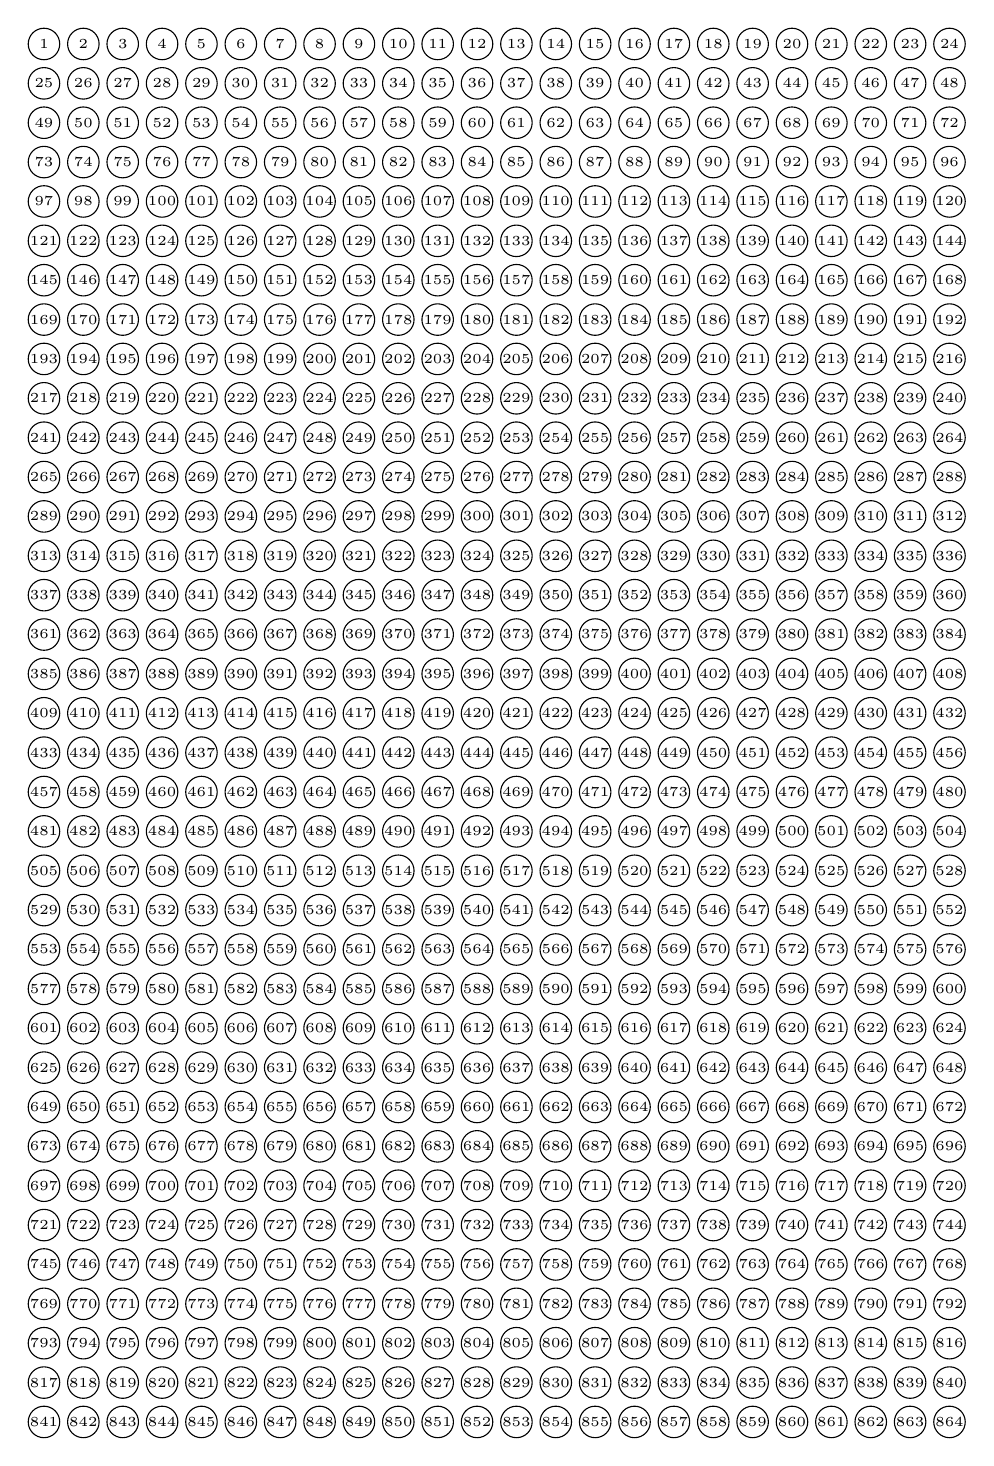
\begin{tikzpicture}[x=0.5cm,y=0.5cm]
        
        % PARAMETERS
        \def\Cols{24}                       % number of columns
        \def\N{864}                        % max number
        \pgfmathsetmacro{\Rows}{ceil(\N/\Cols)}  % computed number of rows
        \def\CirDiam{0.4cm}                 % diameter of every circle
        
        % 1) draw every number in a white circle of fixed size
        \foreach \i in {1,...,\N} {
          \pgfmathtruncatemacro{\c}{mod(\i-1,\Cols)}
          \pgfmathtruncatemacro{\r}{int((\i-1)/\Cols)}
          \node[
          circle,
          draw,
          fill=white,
          minimum size=\CirDiam,
          inner sep=0pt,
          font=\tiny
          ] at (\c+0.5,-\r-0.5) {\i};
        }
        
      \end{tikzpicture}%
    }
  \end{figure*}
  \begin{figure*}[p]
    \centering
    \resizebox{\textwidth}{!}{%
      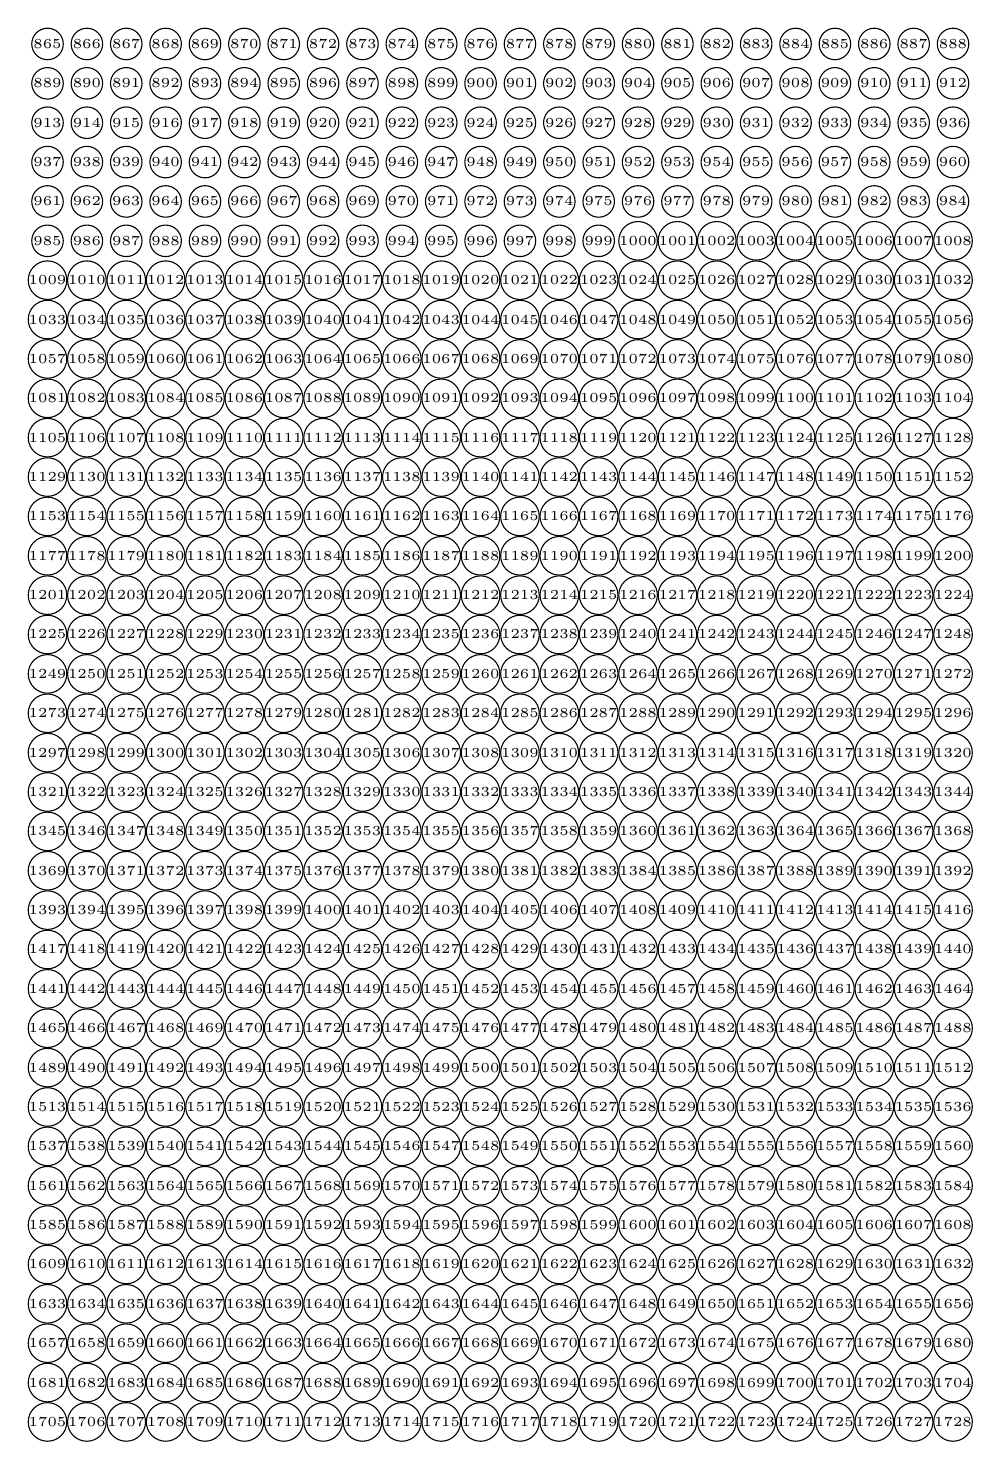
\begin{tikzpicture}[x=0.5cm,y=0.5cm]
        
        % PARAMETERS
        \def\Cols{24}                       % number of columns
        \def\N{864}                        % max number
        \pgfmathsetmacro{\Rows}{ceil(\N/\Cols)}  % computed number of rows
        \def\CirDiam{0.4cm}                 % diameter of every circle
        
        % 1) draw every number in a white circle of fixed size
        \foreach \i in {1,...,\N} {
          \pgfmathtruncatemacro{\c}{mod(\i-1,\Cols)}
          \pgfmathtruncatemacro{\r}{int((\i-1)/\Cols)}
          \pgfmathtruncatemacro{\v}{\N+\i}
          \node[
          circle,
          draw,
          fill=white,
          minimum size=\CirDiam,
          inner sep=0pt,
          font=\tiny
          ] at (\c+0.5,-\r-0.5) {\v};
        }
        
      \end{tikzpicture}%
    }
  \end{figure*}
  \clearpage
}

%%% Local Variables:
%%% mode: latex
%%% TeX-master: "elementary-number-theory"
%%% End:
